Figure \ref{fig:best_class} shows the classification accuracy of
the best models for classification on all $15$ sessions of day
$1$, for SVMs and NNs. The analysis detailed in the previous
Subsection has been repeated for the Neural Network. In that case,
models $8$ and $15$ of day $1$ have been used to build the best
model. Result for day 2 are similar.

\begin{figure} \centering
    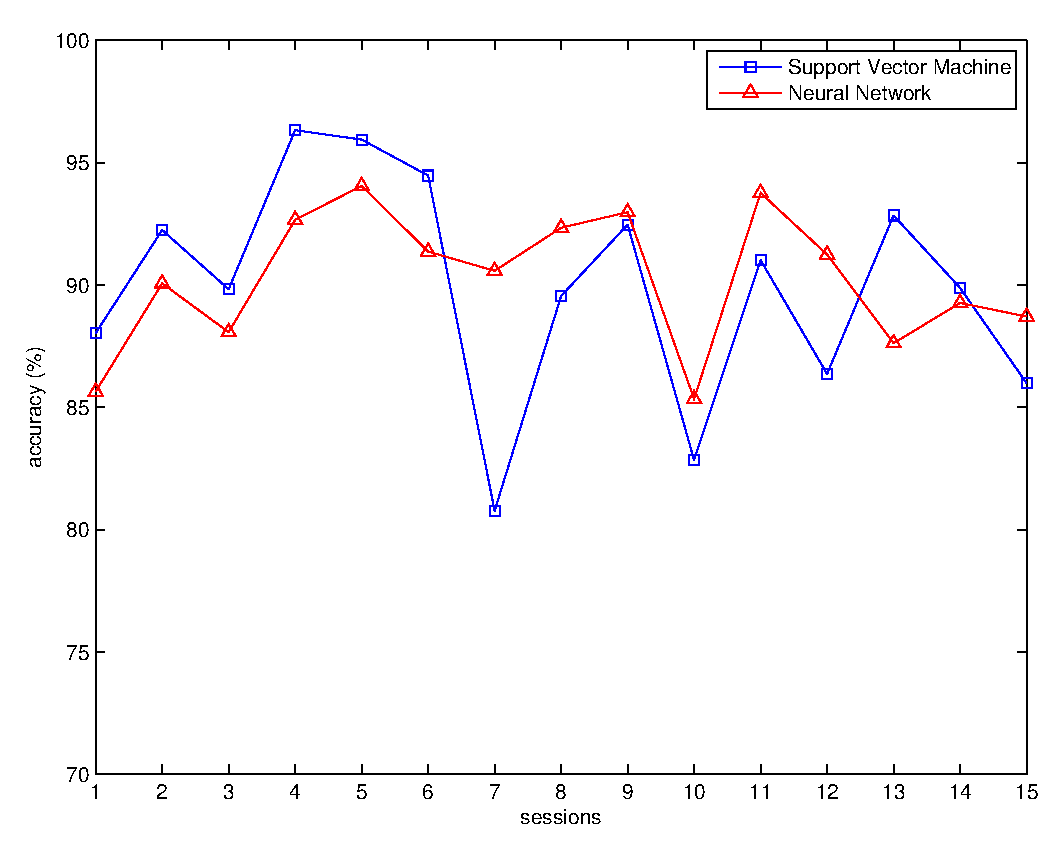
\includegraphics[width=0.4\textwidth]{figs/fig_class_resCrossBestOnDay1} \\
  \caption{Classification accuracy of best models, day $1$. SVM: $89.90\% \pm 4.51\%$;
    NN: $90.25\% \pm 2.77\%$.}
  \label{fig:best_class}
\end{figure}

As one can see, there is no clear winner between SVMs and NNs. NNs
perform slightly better on day $1$ (lower mean, lower standard
deviation) but SVMs are analogously better on day $2$. All in all,
classification accuracy is good, at an overall rate of about
$90\%$. In this case, the training data amounts to four sessions
(uniformised in the case of SVMs and full in the case of NNs), which
is about $12$-$15$ minutes of user activity. But notice, that samples
gathered during both days were necessary to have an idea of which
sessions to use.
